\newchapter{commissioning}{Setup and Commissioning of the PFF System}

This is the introductory text.

\newsection{fontSetup}{Feedforward Controller (FONT5a Board)}

\subsection{Cabling Setup}
\label{ss:fontCables}

\subsection{Implementation of PFF Algorithm in Firmware}
\label{ss:pffFirmware}

Not using arcsin in phase reconstruction - effect

Gain conversion factor

\subsection{DAQ and Setup Parameters}
\label{ss:fontDAQ}

gain
n                                                                                                           
filter weights

timing delays

saturate rather than overflow output

Interleaved mode


\subsection{ADC Droop Correction}
\label{ss:droopCorr}

The droop in the response of the FONT5 ADCs, as most clearly seen in the output of the diode channel in Figure \ref{f:diodeDroop} (although it also effects the mixer channel), is not an issue for the work the FONT group does at ATF2 where the signals are well approximated by delta functions separated by \(\sim\)100~ns. Although the droop has been seen previously, its significance for the continuous microsecond length pulse at CTF3 had not been considered because of this.

\begin{figure}
  \centering
  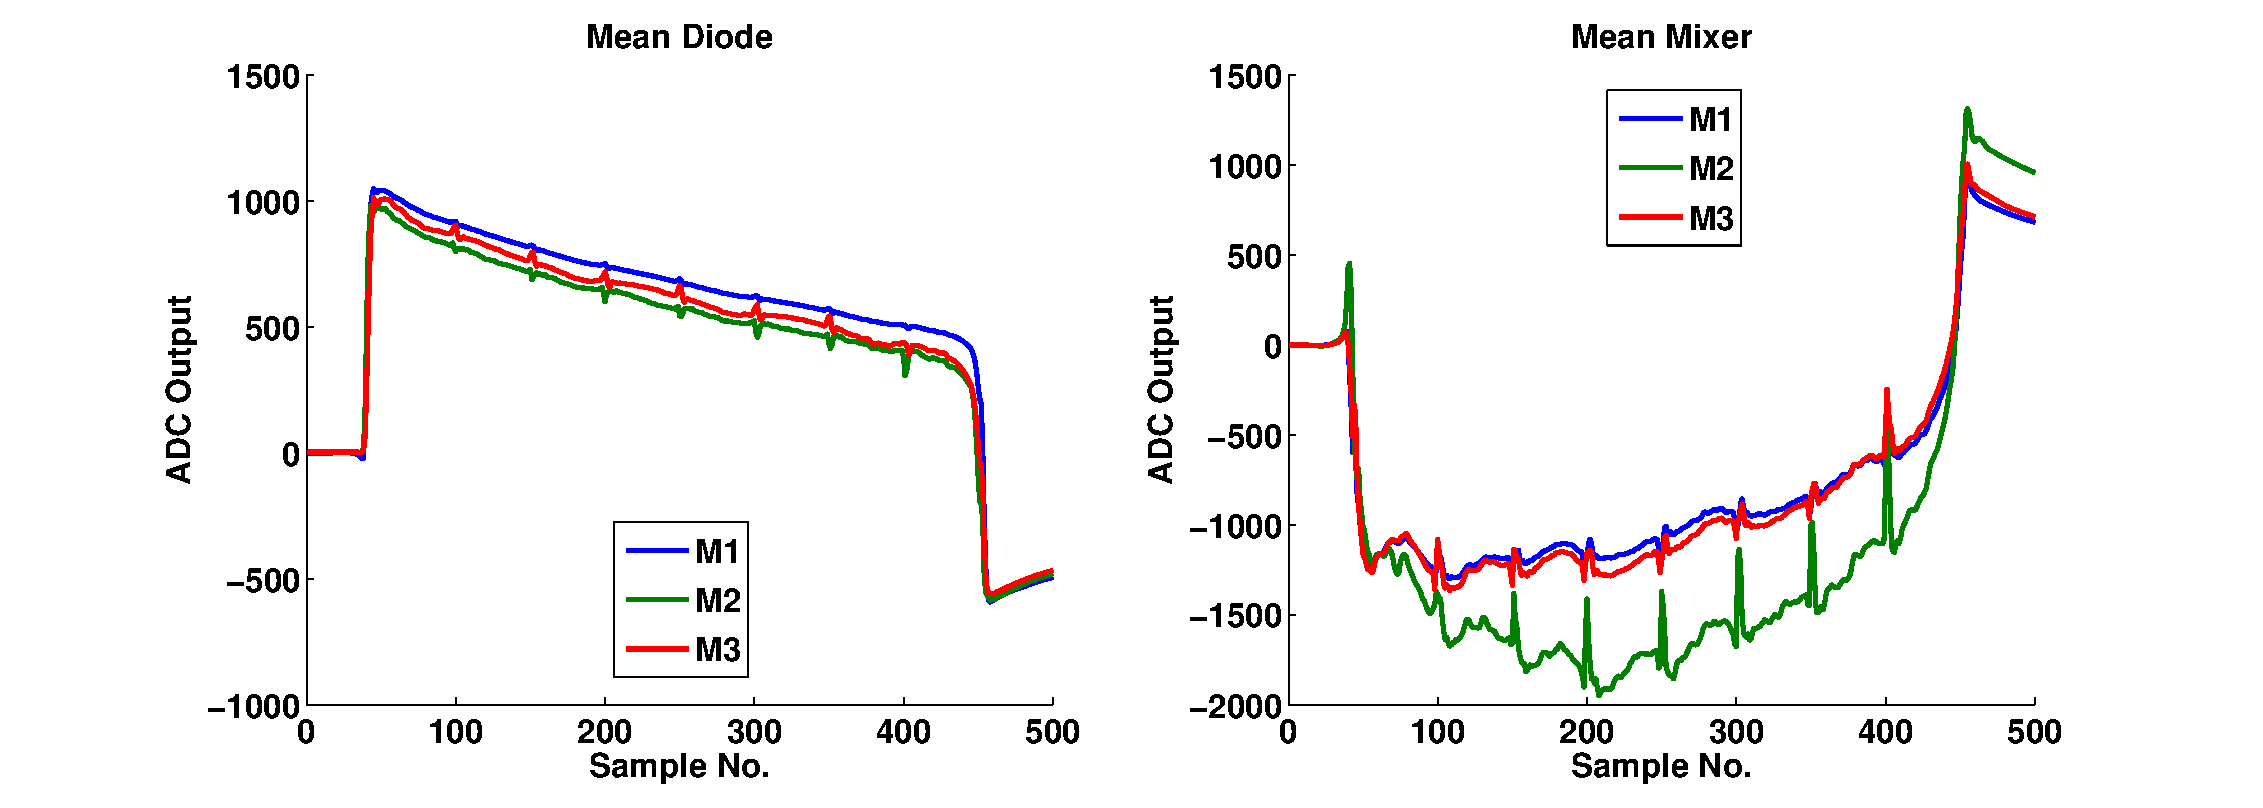
\includegraphics[width=0.9\textwidth]{Figures/commissioning/diodeDroop}
  \caption{Mean diode and mixer output with no filter.}
  \label{f:diodeDroop}
\end{figure}

The droop emerges as a result of the use of AC coupling on the ADC input transformers for electrical isolation. This involves using a capacitor, the current across which is dependent on \({dV}/{dt}\) (\(V\) being voltage and \(t\) time), to remove the DC component from a signal. In particular for the diode channel, which should be a square wave, the output is increasingly well described by a DC signal on the flat top as you move away from the leading edge of the pulse, with the capacitor causing droop in the response as a result.

In the simplest case the droop should be well described by an exponential decay of the form \(A\exp\left(-t/T\right)\). The droop makes it difficult to perform calibrations and measurements on the data and one way in which it could be removed in offline analysis is by determining the decay constants, \(T\), for each of the ADCs on the FONT5 board. To avoid the influence of beam effects tests were done in Oxford using a generated 10~\(\mu\)s DC pulse.

\begin{figure}
  \centering
  \includegraphics[width=0.45\textwidth]{Figures/commissioning/droopFit}
  \caption{Attempted exponential fit to the ADC droop.}
  \label{f:droopFit}
\end{figure}

Unfortunately, as can be seen in Figure \ref{f:droopFit} which shows an example of an exponential fit for one ADC, although the fits return good \(R^{2}\) values it is clear that the slope of the exponential curve is not a good match for the slope of the data. This is perhaps not unexpected as the ferrite cores used in the transformers have many non-linear properties. In fact, by using a fit with two exponential terms it is possible to obtain a perfect match to the data but at this point the complexity of the fit would make any attempt to remove the droop in real beam data in this way spurious.

Instead, changes will be made to the currently in development FONT5a board hardware and firmware to greatly reduce the scale of the droop. Different transformers will be used to reduce the droop rate by up to a factor of fifty and in addition digital filtering will be implemented in firmware to smooth out and reduce the remaining droop component even further. It is expected that after these changes the droop will be small enough to not have a detrimental effect on the performance of the phase feedforward system. 


\newsection{amplifierSetup}{Amplifier}

Make point that all effects here much smaller than phase monitors/phase propagation and although important to highlight them no attempts yet made to correct them or take them in to account in simulations.

Amplifier versions:

First version (nov 2014) 350 V (check)

2nd version  (jul 2015) 650 V - double FETs

3rd version: 1200 V with combiner module (?) not pursued

\subsection{Installation}
\label{ss:ampInstallation}


Amplifier inputs:

Trigger from FONT5a board

DAC1 and DAC2 from FONT5a board


Amplifier outputs:

4 drive signals - one for each strip. Sent to downstream end of kicker (why?)

4 terminators

Amplifier on time monitoring

Monitoring of each amplifier output

\begin{figure}
  \centering
  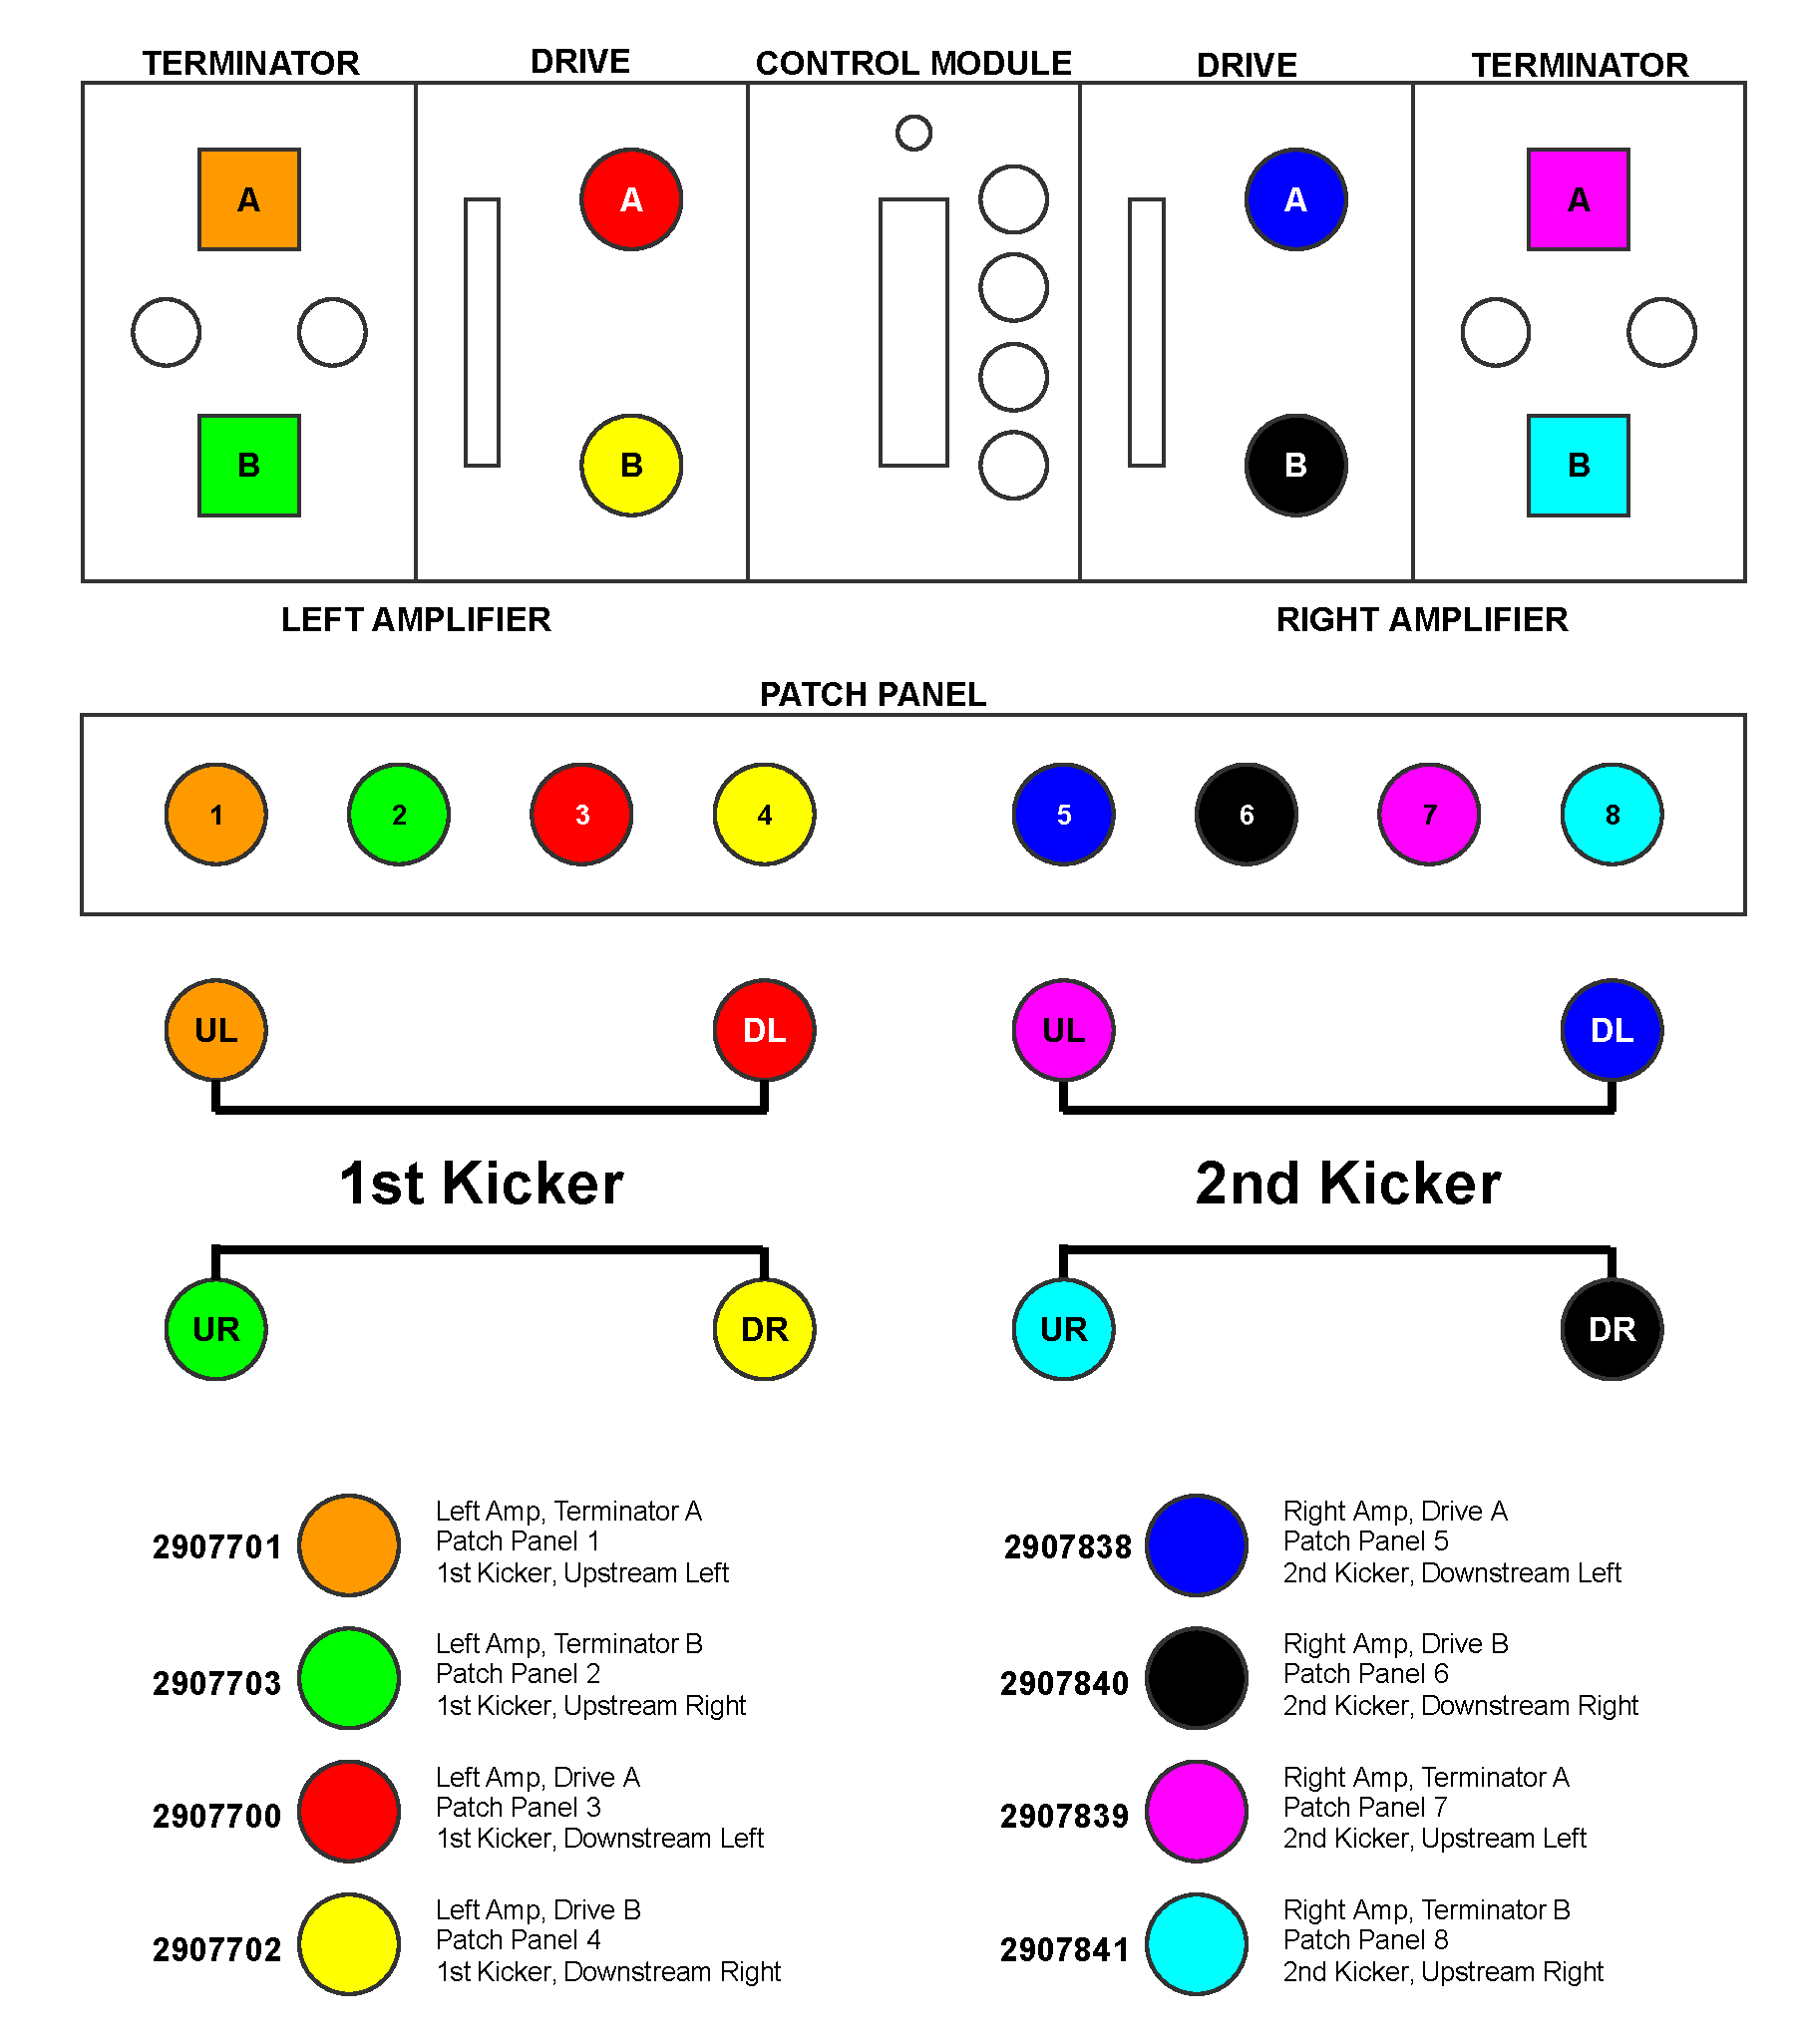
\includegraphics[width=0.9\textwidth]{Figures/commissioning/kickerCables}
  \caption{Cabling setup for cables between the amplifier and kickers.}
  \label{f:kickerCables}
\end{figure}


\subsection{Linearity}
\label{ss:ampLin}

Figure \ref{f:AmpOutvsDAC} shows the amplifier output, as measured by the monitoring signals, at different constant input voltages sent from the FONT5a board between the minimum of -2V (-4096 DAC counts) and maximum of 2V (+4096 DAC counts). The output voltage from the monitoring signals is converted in to the real amplifier output Voltage using the approximate conversion factor of 115. All four amplifier outputs are shown (one for each strip of the two kickers). The plotted values are means taken across a 480~ns central part of the whole 1400~ns output pulse.

The relative polarity of the four outputs is equivalent to what would be sent to the kickers during PFF operation, with opposite polarity of the L and R amplifier outputs sent to each kicker, so that the beam is kicked in opposite directions by each kicker with the second kicker then closing the orbit bump created by the first. Within each side of the amplifier the A and B outputs (sent to each side of the kicker) also have opposite polarity, necessary to create the potential difference across the strips within each kicker that creates the deflecting field for the beam. The relative polarity of the A and B outputs is fixed in the amplifier design and cannot be controlled via the FONT5a board.

The response of the amplifier is highly linear in the region between \(\pm1.2\)~V sent to the amplifier. Outside this range the amplifier clearly begins to enter saturation, in particular above input voltages of \(\pm1.7\)~V. The linear fits shown include only the points between \(\pm1.2\)~V, excluding the first and last three points in the scan of input voltages, in order to not be biased by the effects of saturation.

Figure \ref{f:AmpOutvsDAC_residual} shows the residuals between the linear fit and the real amplifier output across the full range of input voltages. By looking at the residuals a slight deviation from linearity in the \(\pm1.2\)~V range is also visible, although the maximum difference is only 10~V or a 3\% relative error. At the maximum input voltage of \(\pm2\)~V the difference between the real output and the amplitude expected if the response was linear across the full range rises above 150~V, or a relative error of more than 25\%. For example, the RB output at an input voltage of \(+2\)~V is 605~V but the fitted response gives 769~V, a difference of 164~V or 27\%.

The effects of amplifier saturation are not taken in to account in the PFF algorithm on the FONT5a board, in which the DAC output is linearly dependent on the input phase (voltage from the phase monitor mixer signal) across the full range. The applied correction to the downstream phase will therefore be non-optimal when the DAC output calculated by the PFF algorithm is above an absolute value of 2500 counts (1.2~V sent to the amplifier). To date the non-linearity of the amplifier as it begins to enter saturation has also not been included in the PFF simulations presented in the following chapters. This may partially explain the small discrepancies seen between the simulated and real results in some datasets, so including the effect will be pursued in the future. In addition, it could be foreseen to incorporate the saturation characteristics in to the PFF algorithm on the FONT5a board, so that calculated outputs above 2500 counts are boosted slightly to compensate for the lower than expected amplifier output.

Discrepancies between the four amplifier outputs are also visible in Figure \ref{f:AmpOutvsDAC_residual} and Table \ref{t:AmpOutVsDAC}, both in terms of gradient and peak output. This can be partially but not completely explained by errors of up to a few percent in the precise calibration of the four monitoring outputs, which do not output exactly 1/115 of the real input voltage [TODO: Ask Colin about errors]. Differences between the A and B outputs sent to each kicker are not an issue for the PFF performance as both are linear (in the \(\pm1.2\)~V range) and the kick experienced by the beam in each kicker is proportional to the difference of the two. Therefore, only the calibration between the output from the FONT5a board sent to the amplifier and the resulting phase shift in the TL2 chicane is affected. However, disparity between the potential difference across each kicker (LA-LB and RA-RB), so that the deflection of the beam in each kicker is different, leads to the orbit bump created by the PFF system not being closed in the chicane, degrading the horizontal beam stability downstream. The fitted potential difference at 1~V input is 869~V for the left amplifier (LA-LB, sent to the first kicker) and 835~V for the right amplifier (RA-RB, sent to the second kicker), a difference of 4\%. This can be compensated in the PFF setup on the FONT5a board by using a different gain for each correction output, so that the voltage sent to the right amplifier is higher but the resulting output voltage sent to both kickers is the same. Orbit closure is discussed further in Section \ref{ss:orbitClosure}.


\begin{figure}
  \centering
  \includegraphics[width=0.9\textwidth]{Figures/commissioning/AmpOutvsDAC}
  \caption{Amplifier output vs. input.}
  \label{f:AmpOutvsDAC}
\end{figure}

\begin{figure}
  \centering
  \includegraphics[width=0.9\textwidth]{Figures/commissioning/AmpOutvsDAC_residual}
  \caption{Residual between amplifier output and linear fit.}
  \label{f:AmpOutvsDAC_residual}
\end{figure}

\begin{table}
  \begin{center}
    \begin{tabular}{| c | c |}
	   \hline
       Amplifier Port & Output at +1~V Input \\ \hline
       LA & \(+416\pm3\)~V \\
	   LB & \(-453\pm3\)~V \\
	   RA & \(-426\pm3\)~V \\
	   RB & \(+409\pm3\)~V \\
 	   \hline
    \end{tabular}
    \caption{Feedforward results using combined data from 20th November 2015.}
  	\label{t:AmpOutVsDAC}
  \end{center}
\end{table}

\subsection{Shape}
\label{ss:ampShape}

In the previous section the linearity of the mean output was considered but the performance of the PFF correction is clearly also sensitive to any variations in output voltage along the amplifier output pulse. Figures \ref{f:ampLTraces} and \ref{f:ampRTraces} show the full 1.4~\(\mathrm{\mu}\)s amplifier output pulse at a constant \(+1\)~V input sent to the left amplifier and a constant \(-1\)~V input sent to the right amplifier respectively. Spikes in the signal just prior to 2000~ns and after 3000~ns on the time axis as seen in the plots are beam pickup induced by the beam passing through the kickers. These are therefore not a property of the amplifier performance and are excluded from the analysis in this section. However, the beam pickup is used later in Section \ref{ss:absTiming} for the purposes of optimising the correction timing.

\begin{figure}
  \centering
  \includegraphics[width=0.9\textwidth]{Figures/commissioning/AmpL_Traces}
  \caption{Amp L along pulse at 1 V input}
  \label{f:ampLTraces}
\end{figure}

\begin{figure}
  \centering
  \includegraphics[width=0.9\textwidth]{Figures/commissioning/AmpR_Traces}
  \caption{Amp R along pulse at 1 V input}
  \label{f:ampRTraces}
\end{figure}

For each side of the amplifier both the A and B outputs are plotted as well as the difference of the two, which is the relevant quantity in terms of the kick received by the beam as it traverses the kickers. In the ideal case the potential difference should be flat along the full pulse length. However, for both the left and right side variations in the difference are visible, with an initial increase in output across the first 500~ns of the pulse followed by a droop in response across the second half of the pulse. Although not shown here, the shape of the variations along the pulse is consistent across the full range of output voltages, and scale in magnitude with the output voltage. Figure \ref{f:ampFlatness} shows the peak-to-peak and mean deviation of the output voltage along the pulse across the full range of input voltages. The peak-to-peak deviation refers to the difference between the minimum and maximum output along the pulse, whilst the mean deviation is the average absolute difference between the mean output and the output at each sample point. For a constant input voltage the output voltage along the pulse varies by up to 88~V peak-to-peak (mean 12~V) for the left amplifier or 93~V peak-to-peak (mean 14~V) for the right amplifier. As a relative difference, this corresponds to approximately a 6~\% peak-to-peak, or 1~\% mean, variation along the pulse.

The PFF algorithm on the FONT5a board uses a single gain value across the whole pulse length for each correction output, thus making the approximation that the amplifier response is flat along the pulse. The variations along the amplifier pulse therefore directly translate in to discrepancies between the intended phase shift as calculated and the real phase shift experienced by the beam. As the region of interest for the correction is a few hundred nanoseconds about the central part of the pulse, as opposed to the full pulse length, the 1~\% mean variation is more indicative of the resulting error than the 6~\% peak-to-peak variation. With a correction range (Section \ref{ss:corrRange}) of \(\pm6^\circ\), the effects of the non-flat amplifier output should be below \(0.06^\circ\) and not measurable considering the phase monitor resolution of \(0.14^\circ\). Nevertheless, it could be foreseen to implement a droop correction in the PFF algorithm on the FONT5a board, taking the variations in the amplifier output along the pulse in to account.

\begin{figure}
  \centering
  \includegraphics[width=0.9\textwidth]{Figures/commissioning/AmpFlatness}
  \caption{Flatness of potential difference sent to kickers.}
  \label{f:ampFlatness}
\end{figure}

As for the mean output voltage, the second way variations in the amplifier output along the pulse can impact the PFF performance is via the orbit closure in the chicane. For this the relevant quantity is the sum of the potential difference sent to each kicker, or \((LA-LB)+(RA-RB)\). To ensure orbit closure this quantity, named the residual kick here, should be zero across the whole pulse length for all input voltages. Figure \ref{f:ampClosure} shows the residual kick along the pulse for all the input voltages in the scan. Clearly they are not all centred around zero, but this is expected due to the differences in the mean output voltage of the four amplifier outputs seen in the previous section. As already stated, the overall mean offset can be removed by using a different gain for the two correction outputs. However, any variations along the pulse cannot be compensated for in the PFF algorithm. The magnitude of the effect is summarised in Figure \ref{f:ampClosureFlatness}, showing the peak-to-peak and average deviation of the residual kick from flat. The overall residual kick is very flat and effect is smaller than any of those previously shown --- only up to 2~V on the mean or 21~V peak-to-peak. Whether this has any measurable effect on the orbit closure is discussed in Section \ref{ss:orbitClosure}.

\begin{figure}
  \centering
  \includegraphics[width=0.9\textwidth]{Figures/commissioning/residualKick_Traces}
  \caption{Residual kick along pulse.}
  \label{f:ampClosure}
\end{figure}

\begin{figure}
  \centering
  \includegraphics[width=0.9\textwidth]{Figures/commissioning/residualKick_Flatness}
  \caption{Residual kick along pulse: deviation from flat.}
  \label{f:ampClosureFlatness}
\end{figure}

\subsection{Bandwidth}
\label{ss:ampBand}

\newsection{daqSigProc}{Data Acquisition and Signal Processing}

\subsection{SiS Digitiser Setup}
\label{ss:sisSetup}

(already discussed in ph mon chapter)

\subsection{Acquisition Tools}
\label{ss:acqTools}

\subsection{Monitoring Tools}
\label{ss:monTools}

Online display

\subsection{Time Alignment of Signals}
\label{ss:timeAlignment}

\subsection{Definition of Zero Phase}
\label{ss:zeroPhase}

\newsection{constKicks}{Kicker and Optics Performance Verification}

\subsection{Correction Range}
\label{ss:corrRange}

http://accelconf.web.cern.ch/accelconf/ipac2011/papers/tupc007.pdf
1.4 kV to each strip = 1 mrad kick at 150 MeV
1.26 kV to each strip = 1 mrad kick at 135 MeV


Scan and comparison to expectation from optics.

Effect on correction.

Optics: 0.7m R52 -> 10 degrees for 1mrad kick


\subsection{Linearity}
\label{ss:kickLin}

\subsection{Orbit Closure}
\label{ss:orbitClosure}

\subsection{Shape}
\label{ss:kickShape}

Shape of FF kick on BPMs vs. shape of upstream phase

\newsection{timing}{Correction Output Timing}

\subsection{Latency}
\label{ss:measLatency}

\subsection{Absolute Timing}
\label{ss:absTiming}

\subsubsection{Using Beam Pickup}
\label{sss:beamPickup}

\subsubsection{Using BPMs}
\label{sss:relativeBPM}

\subsection{Relative Kicker Timing}
\label{ss:relativeTiming}

\begin{figure}
  \centering
  \includegraphics[width=0.45\textwidth]{Figures/commissioning/relativeTimingScan_traces}
  \caption{Traces relative timing scan.}
  \label{f:relativeTimingScan_traces}
\end{figure}

\begin{figure}
  \centering
  \includegraphics[width=0.45\textwidth]{Figures/commissioning/relativeTimingScan_slopeFit}
  \caption{Relative timing scan - fit to rising/falling edge.}
  \label{f:relativeTimingScan_slopeFit}
\end{figure}



%\newsection{corrBandwidth}{Correction Bandwidth}




